\documentclass[11pt]{article}
\usepackage{hyperref}
\usepackage[utf8]{inputenc}
\usepackage{graphicx}

\title{NLP-2024-A3: Poem Generator}
\author{Fei Huang[2818760]}
\date{\today}

\begin{document}

\maketitle

\section{Introduction}

The Poem Generator (Web App) is designed to inspire users by generating poems based on personalized inputs. This application allow users to specify emotions and styles as well, combining NLP technology with the classical art of peotry to conduct a preliminary study on creative expression.

\section{Code Overvies}

\textbf{GitHub Repo Link:} \url{https://github.com/huangf06/NLP_2024_A3}

The application is built on the Flask web framework, structured around a central Python script, \texttt{app.py}, which handles routing and server-side logic. The backend uses the \texttt{transformers} library to build a pre-trained NLP model, faciilitating the generations of poems based on user input. After multiple parameter adjustments, we ultimately achieved a relatively satisfactory model.

\section{Application Functionality and Screenshots}

\begin{figure}[ht]
\centering
% Adjust the width as needed to fit them side by side and align their tops
\raisebox{-\height}{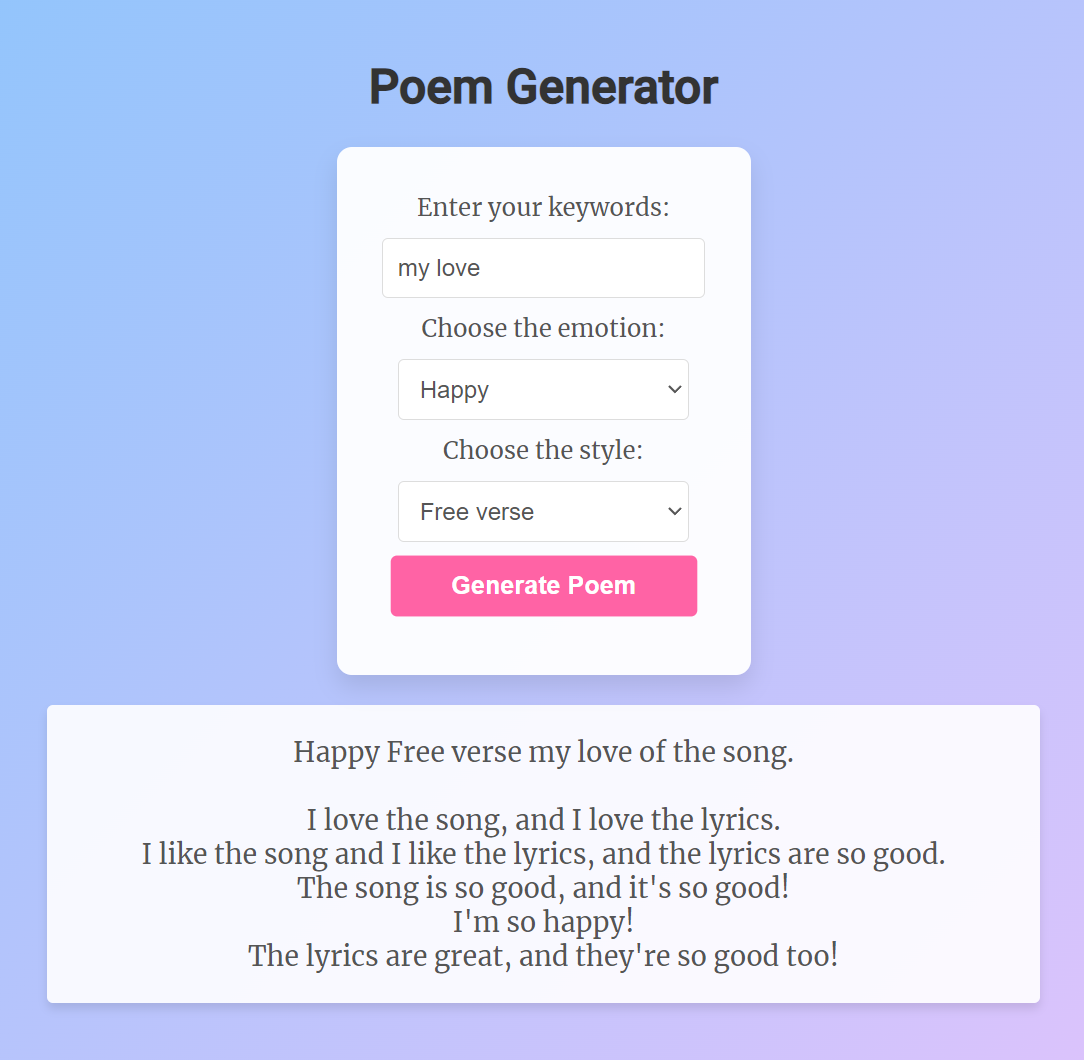
\includegraphics[width=0.45\textwidth]{pic/screenshot1.png}}
\hfill % Ensures that there is no additional space if the images do not fill the line
\raisebox{-\height}{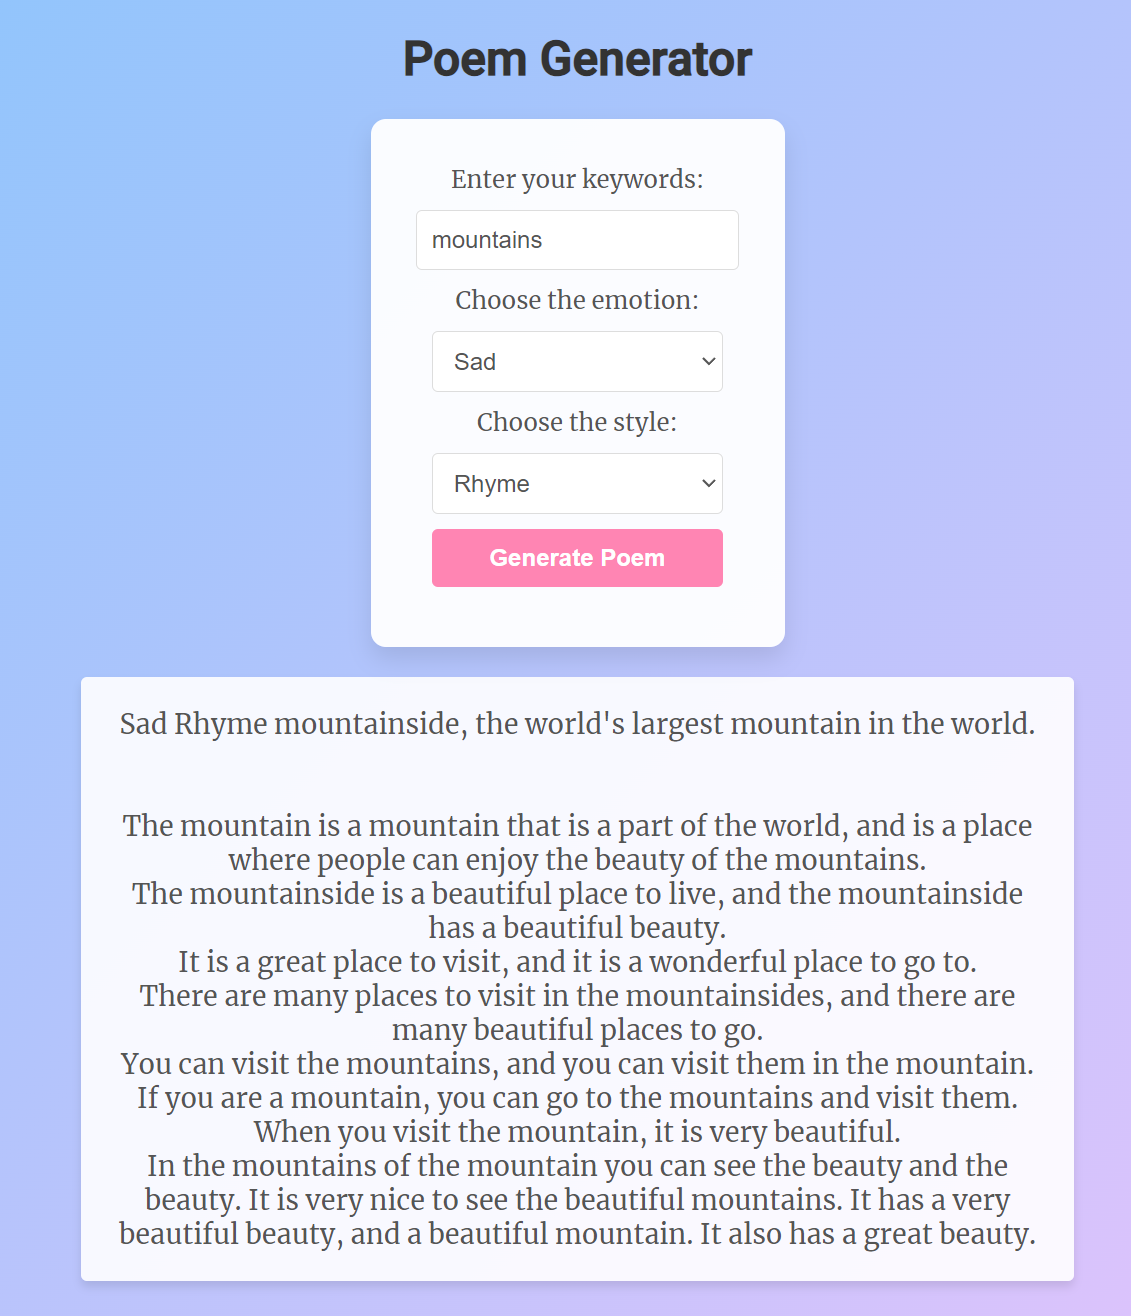
\includegraphics[width=0.45\textwidth]{pic/screenshot2.png}}
\caption{Screenshots of User Interface}
\end{figure}

\textbf{Input:} Users begin by entering keywords that set the theme of the poem. They then select an emotion and a style from dropdown menus, choices that guide the tone and structure of the generated poetry.

\textbf{Processing:} Once the input is submitted, the backend processes this data using a combination of Flask routing and NLP model inference. The chosen keywords and attributes influence the poem's generation logic, implemented via the \texttt{transformers} library.

\textbf{Output:} The poem is dynamically generated and displayed on the same page, allowing users to immediately see the result of their choices.



\section{Linguistic Significance}

\textbf{NLP Techniques:} The application utilizes a pre-trained model from the \texttt{transformers} library, specifically chosen for its capability to understand context and generate coherent text. This model is based on the GPT-2 architecture, which balances between advanced linguistic capabilities and computational efficiency. In the development process of our model, we repeatedly adjusted parameters and refined the logic to reduce repetition and improve output reasonableness. This iterative optimization was critical for enhancing the quality and creativity in the text produced. 

\textbf{Educational Value:} The Poem Generator serves not only as a tool for entertainment but also as an educational platform where uses can explore the impact of different choices on text generation. It can be used in educational settings to demonstrate the application of machine learning in creative writing and linguistics.

\section{Collaborative Work Disclosure}

\textbf{Collaboration Details:} This project was developed individually, with additional support from GPT4 in adjusting the frontend interface.

\begin{thebibliography}{99}

\bibitem{radford2019language}
Alec Radford, Jeffrey Wu, Rewon Child, David Luan, Dario Amodei, Ilya Sutskever.
\textit{Language Models are Unsupervised Multitask Learners}.
2019.
\url{https://cdn.openai.com/better-language-models/language_models_are_unsupervised_multitask_learners.pdf}

\bibitem{vaswani2017attention}
Ashish Vaswani, Noam Shazeer, Niki Parmar, Jakob Uszkoreit, Llion Jones, Aidan N Gomez, Lukasz Kaiser, Illia Polosukhin.
\textit{Attention is all you need}.
In \textit{Advances in neural information processing systems}, pages 5998--6008.
2017.

\bibitem{brown2020language}
Tom B Brown, Benjamin Mann, Nick Ryder, Melanie Subbiah, Jared Kaplan, Prafulla Dhariwal, Arvind Neelakantan, Pranav Shyam, Girish Sastry, Amanda Askell, et al.
\textit{Language Models are Few-Shot Learners}.
\textit{arXiv preprint arXiv:2005.14165}.
2020.

\bibitem{goodfellow2016deep}
Ian Goodfellow, Yoshua Bengio, Aaron Courville.
\textit{Deep Learning}.
MIT Press.
2016.
\url{http://www.deeplearningbook.org/}

\bibitem{huggingface2020transformers}
Hugging Face.
\textit{Transformers: State-of-the-art Natural Language Processing}.
2020.
\url{https://huggingface.co/transformers/}

\end{thebibliography}

\end{document}

